\appendix
\pagenumbering{Roman}
\section{Appendix}

\subsection{Additional Figures}
We plot Figures that enhance our line of argumentation but would disturb the train of reading within the main section.
\subsubsection{Piecewise constant results}
\label{A:piecewise}
Figure \ref{fig:results_piecewise_numbers} provides a visualization of our core results for the number of deceased individuals using piecewise constant vaccination channels as functional form of $f_l$. The values do qualitatively not differ form the corresponding spline values depicted in the main text in Figure \ref{fig:results_splines_numbers}. Even the percentage improvement of the unrestricted and the Pareto strategy equal the numbers from the spline analysis. Since the current strategy is no affected by the type of the vaccination channel, it yields the exact same results as within Figure \ref{fig:results_splines_numbers}. For the optimized strategies numbers are slightly shifted between countries, such that country A experiences between 10,000-30,000 more and country B fewer deaths. 
\begin{figure}[h!]
\centering
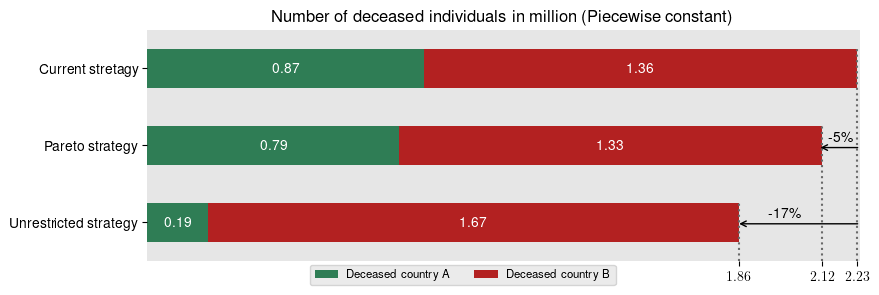
\includegraphics[scale=0.65]{images/piecewise_percentage_deviation.png}\\
\begin{flushleft}
\scriptsize{Note: The numbers within the boxes indicate the number of deceased individuals in million with respect to the respective country and strategy. Numbers at the x-axis represent the total number of deceased individuals within one country. The percentage numbers indicate the change relative to the optimal strategy, e.g. $-5\%$ indicates that by implementing the Pareto strategy 5\% less individuals died in comparison to the current strategy.}
\end{flushleft}
\caption{Number of deceased individuals by country (Stepwise)}
\label{fig:results_piecewise_numbers}
\end{figure}

Figure \ref{fig:results_piecewise_allocation} depicts the optimal doses of vaccine inflow using piecewise constant vaccination channels as functional form of $f_l$. As for the number of deceased individuals, the values do qualitatively not differ form the corresponding spline values depicted in the main text in Figure \ref{fig:results_splines_allocation}. We observe the same strategy for the unrestricted strategy, that nearly assigns no vaccine to country B but only between week 5-9. However, the peak is not as large as in Figure \ref{fig:results_splines_allocation}. As opposed to Figure \ref{fig:results_splines_allocation}, there is no allocation of vaccines to country B at the very beginning, which could explain the higher number of death cases in country B using the stepwise vaccination channel. \\

\begin{figure}[h!]
\centering
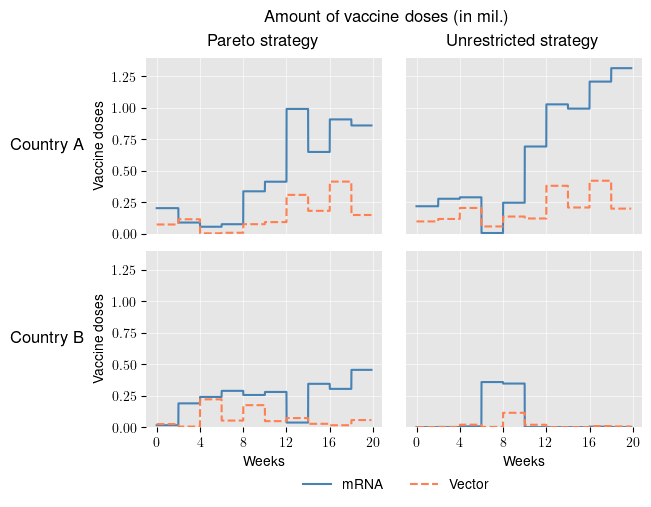
\includegraphics[scale=0.65]{images/piecewise_vaccine_total_quantity.png}\\
\begin{flushleft}
\scriptsize{Note:} Every column represents one vaccination strategy and every row represents one country. Both vaccines are indicated by their colors that are used throughout the paper. 
Every curve is the product of a piecewise constant vaccine inflow and a spline. Thus, the lines appear to be discontinuous piecewise polynomials. 
\end{flushleft}
\caption{Number of allocated vaccine doses (Stepwise)}
\label{fig:results_piecewise_allocation}
\end{figure}

In Figure \ref{fig:results_piecewise_infectious_dead}, we trace out the trajectories of the number of infectious and deceased individuals according to the respective strategies (columns) and countries (rows). The values do qualitatively not differ form the corresponding spline values depicted in the main text in Figure \ref{fig:results_splines_infectious_dead}.\\

\begin{figure}[h!]
\centering
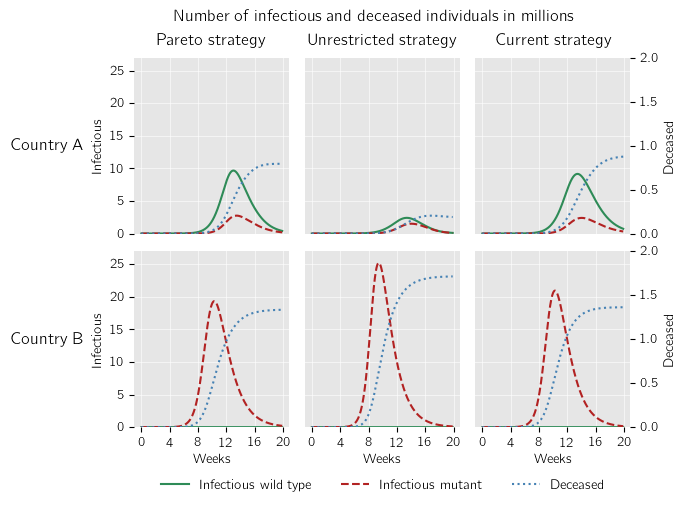
\includegraphics[scale=0.65]{images/piecewise_infectious_dead.png}\\
\begin{flushleft}
\scriptsize{Note:} Every column represents one vaccination strategy and every row represents one country. Every vaccine is indicated by its color that is used throughout the paper. The left y-axis is used for the number of infectious individuals (solid green and dashed red curves). The right y-axis corresponds to the number of deceased individuals (dotted blue line). Both viruses are associated with the color we have used throughout the paper. 
\end{flushleft}
\caption{Number of infectious individuals (Stepwise)}
\label{fig:results_piecewise_infectious_dead}
\end{figure}

\clearpage
\subsubsection{Vaccination allocation fractions}
\label{A:fractions}

Figure \ref{fig:results_piecewise_allocation_fractions} depicts the course of $f_l$ over the whole decison period using a piecewise vaccination channel. Figure \ref{fig:results_splines_allocation_fractions} depicts the respective values for the spline vaccination channels. The values are the quotient of the curve of the vacicne inflow in \ref{fig:available_vaccine} and the optimal total number of vaccine doses inflow in Figure \ref{fig:results_piecewise_allocation} and Figure \ref{fig:results_splines_allocation}.
\begin{figure}[h!]
\centering
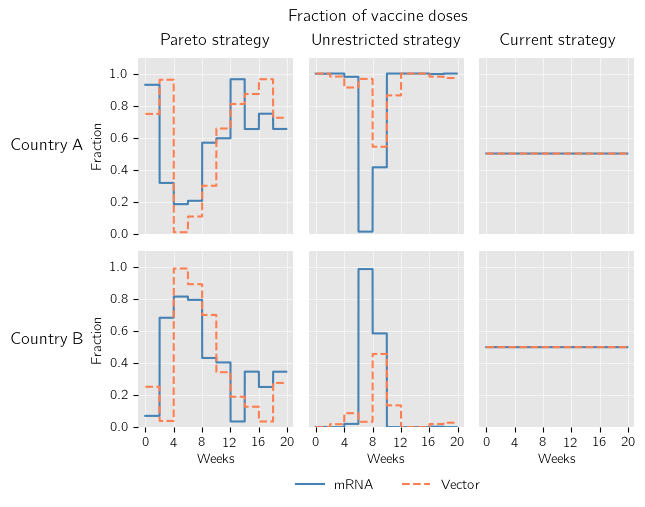
\includegraphics[scale=0.85]{images/piecewise_vaccine_fractions.png}\\
\begin{flushleft}
\scriptsize{Note:} Every column represents one vaccination strategy and every row represents one country. Both vaccines are indicated by their colors that are used throughout the paper. 
\end{flushleft}
\caption{Fractions of vaccines (Stepwise)}
\label{fig:results_piecewise_allocation_fractions}
\end{figure}

\begin{figure}[h!]
\centering
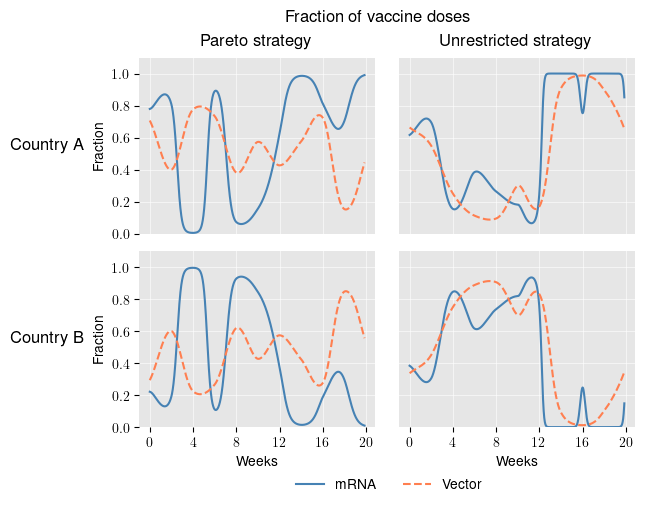
\includegraphics[scale=0.85]{images/splines_vaccine_fractions.png}\\
\begin{flushleft}
\scriptsize{Note:} Every column represents one vaccination strategy and every row represents one country. Both vaccines are indicated by their colors that are used throughout the paper. 
\end{flushleft}
\caption{Fractions of vaccines (Splines)}
\label{fig:results_splines_allocation_fractions}
\end{figure}

\clearpage
\subsubsection{Waterfall plots of optimization}
\label{A:waterfall}
Figure \ref{fig:results_piecewise_waterfall} and Figure \ref{fig:results_splines_waterfall} show the 20 best optima of the multi-start optimization runs. We find that the descend is rather continuous and the optimal values are obtained only once. Hence, it might be possible to find even lower values using more multi-start runs.
\begin{figure}[h!]
\centering
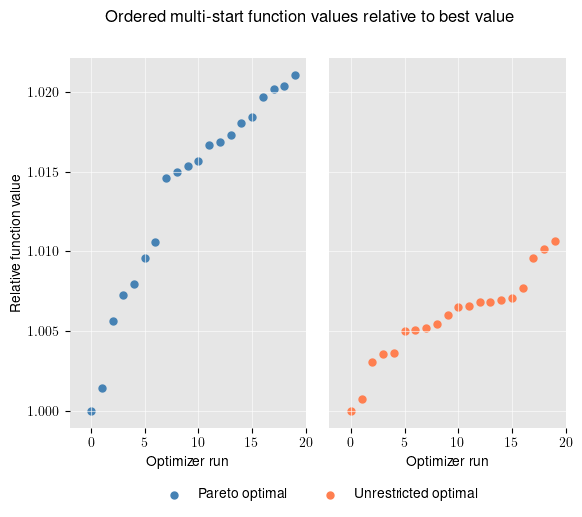
\includegraphics[scale=0.53]{images/piecewise_waterfall.png}\\
\begin{flushleft}
\scriptsize{Note:} Values are relative to the start yielding the lowest optimal minimum value. Only the best 20 starts are used to increase readability. 
\end{flushleft}
\caption{Waterfall plot of the 20 best multi-start runs (Stepwise)}
\label{fig:results_piecewise_waterfall}
\end{figure}


\begin{figure}[h!]
\centering
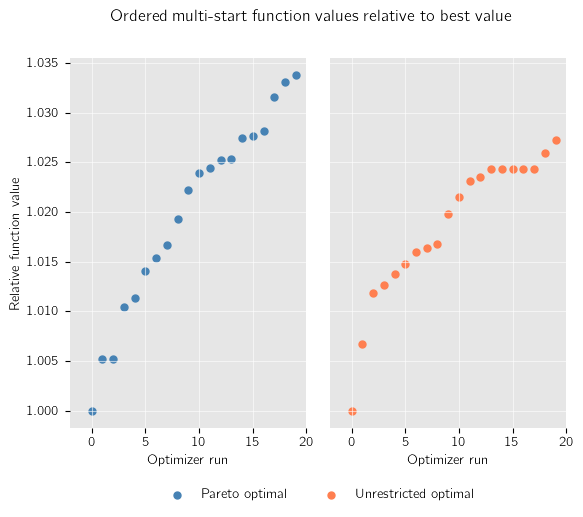
\includegraphics[scale=0.53]{images/splines_waterfall.png}\\
\begin{flushleft}
\scriptsize{Note:} Values are relative to the start yielding the lowest optimal minimum value. Only the best 20 starts are used to increase readability. 
\end{flushleft}
\caption{Waterfall plot of the 20 best multi-start runs (Splines)}
\label{fig:results_splines_waterfall}
\end{figure}

\clearpage
\subsubsection{Simulated distribution of number of deceased individuals}
\label{A:simulated_distr}

Figure \ref{fig:results_piecewise_stochastic_histogram} plots the results for the number of deceased individuals using piecewise constant vaccination channels. We decided to remove it from the main text since the results resemble the results from the spline vaccination channel within Figure \ref{fig:results_splines_stochastic_histogram} in the main section.
\begin{figure}[h!]
\centering
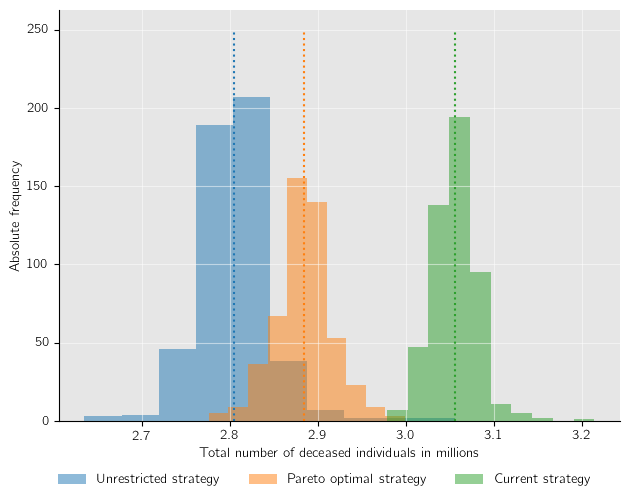
\includegraphics[scale=0.65]{images/piecewise_stochastic_histogram.png}\\
\begin{flushleft}
\scriptsize{Note:} Dotted lines are sample means. The total number of deceased individuals of a strategy is the sum of the respective number of deaths in in country A and country B. We draw 500 samples per strategy. 
\end{flushleft}
\caption{Stochastically observed frequencies (Piecewise)}
\label{fig:results_piecewise_stochastic_histogram}
\end{figure}

Figure \ref{fig:results_piecewise_infectious_dead_stochastic} plots the total number of infectious individuals simulated using the stochastic model. We decided to remove it from the main text since the results resemble the results from the spline vaccination channel within Figure \ref{fig:results_splines_infectious_dead_stochastic} in the main section.\\

\begin{figure}[h!]
\centering
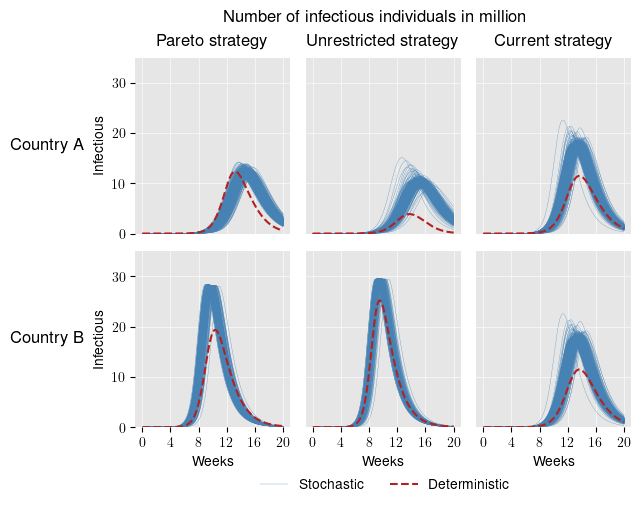
\includegraphics[scale=0.85]{images/piecewise_stochastic_infectious.png}\\
\begin{flushleft}
\scriptsize{Note:} Every column represents one vaccination strategy and every row represents one country. The thin blue lines depict all 500 simulations of the stochastic algorithm using the respective strategy. The dashed red depicts the respective infections within the deterministic model. 
\end{flushleft}
\caption{Number of infectious individuals using Stochastic simulations (Stepwise)}
\label{fig:results_piecewise_infectious_dead_stochastic}
\end{figure}

Figures \ref{fig:histograms_piecewise}  and \ref{fig:histograms_piecewise} depict the 2-dimensional, as well as the marginal, histograms of the number of deceased individuals with respect to the countries. As for the results shown within the main section, the results are qualitatively highly similar. It is striking that for the unrestricted case, the case with the fewest deaths, points seem to fluctuate more random around the center point mass as for the Pareto optimal and the current strategy. For the current strategy and the optimal strategy the reasoning might be that, just by chance, some simulated pandemics result in overall more deaths and therefore both countries have increased numbers in death cases. However, the same reasoning could apply for the unrestricted strategy that shows no linear correlation.
Further research is needed to examine if this patterns occurred randomly and if no what the cause is.
\begin{figure}[h!]
     \centering
     \begin{subfigure}[b]{0.49\textwidth}
         \centering
         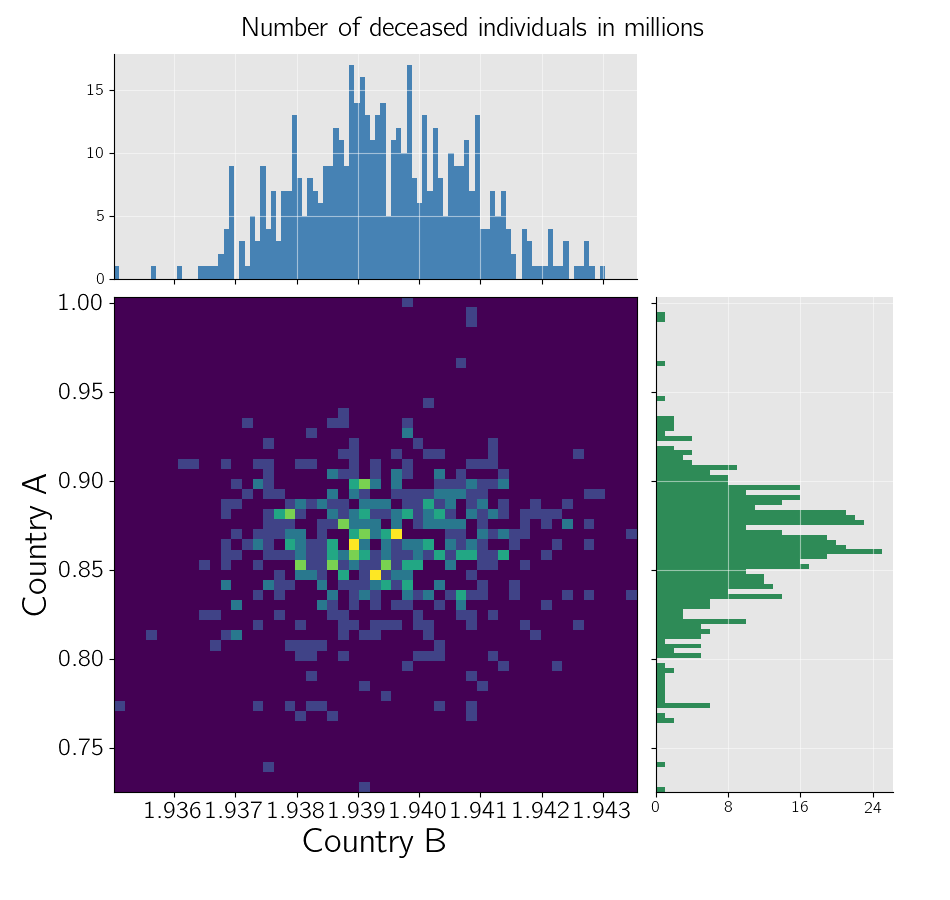
\includegraphics[width=\textwidth]{images/splines_stochastic_histogram_deceased_unrestricted.png}
         \caption{Unrestricted strategy}
         \label{fig:2d_unrestricted}
     \end{subfigure}
     \hfill
     \begin{subfigure}[b]{0.49\textwidth}
         \centering
         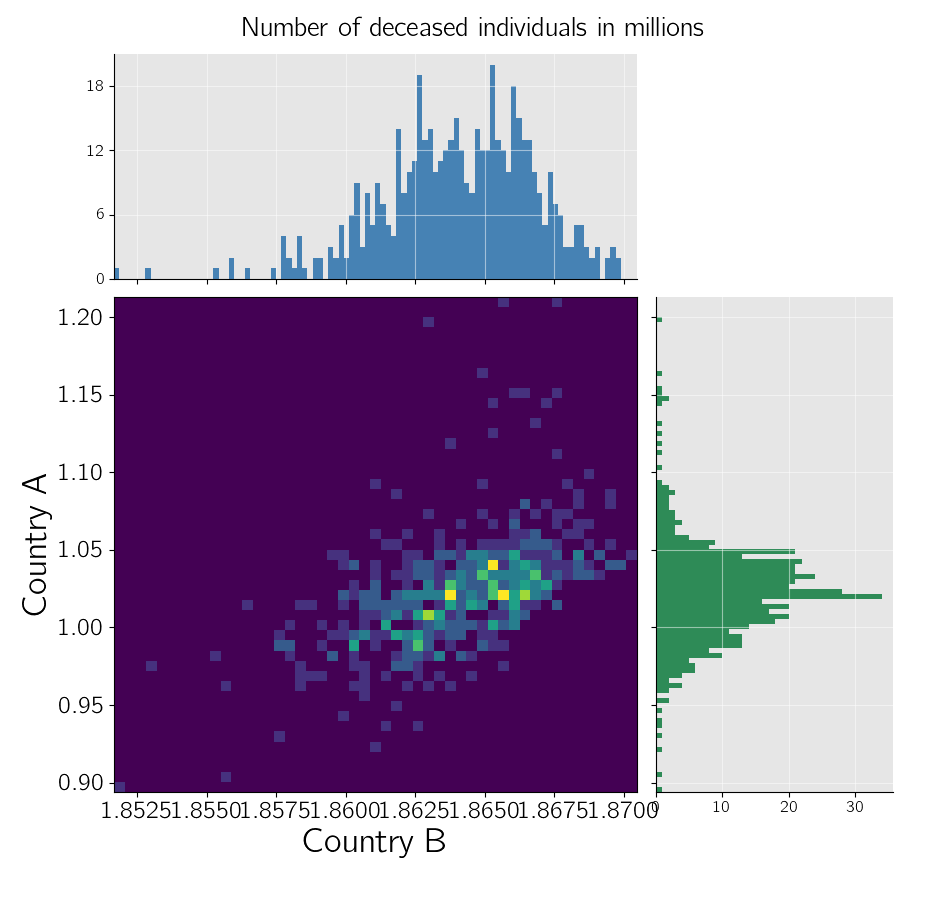
\includegraphics[width=\textwidth]{images/splines_stochastic_histogram_deceased_optimal.png}
         \caption{Pareto optimal strategy}
         \label{fig:2d_optimal}
     \end{subfigure}
     \\
     \begin{subfigure}[b]{0.49\textwidth}
         \centering
         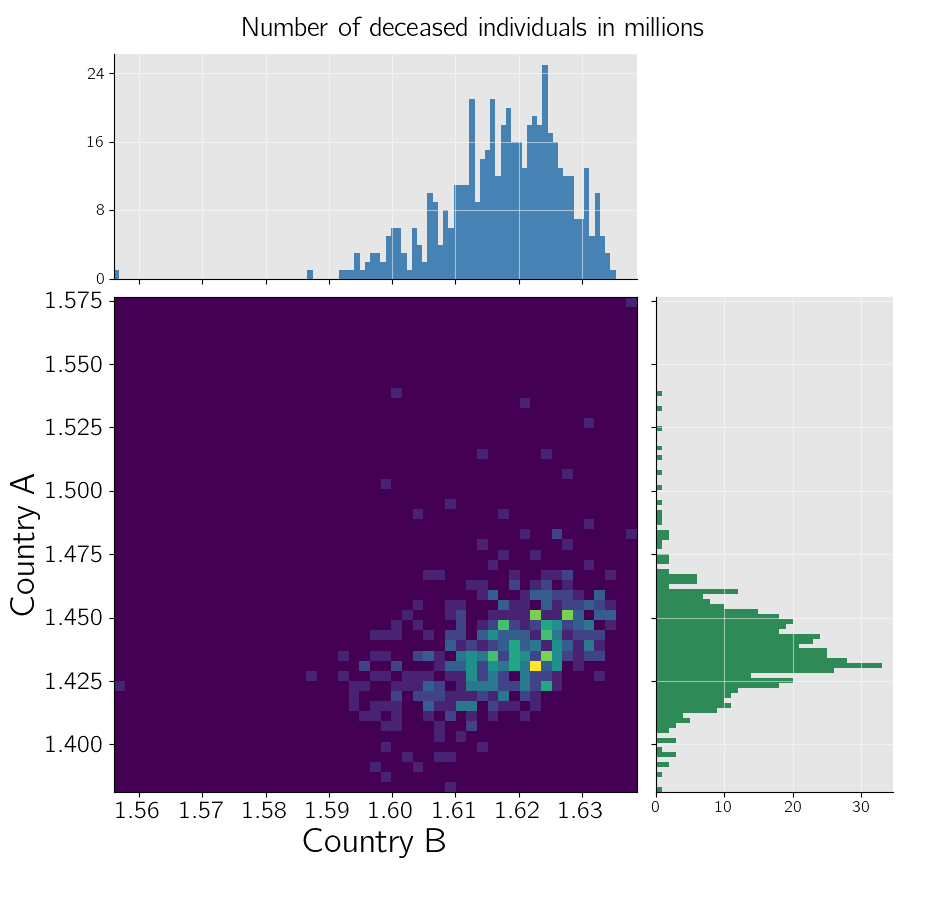
\includegraphics[width=\textwidth]{images/splines_stochastic_histogram_deceased_current.png}
         \caption{Current strategy}
         \label{fig:2d_current}
     \end{subfigure}
\begin{flushleft}
\scriptsize{Note:} Purple temperature boxes indicate the joint frequencies. Histograms on top are the histograms corresponding to country B and histograms at the right-hand side are the histograms corresponding to country A. Histograms are computed using 500 simulations of the stochastic model using the Policies derived from splines. 
\end{flushleft}
        \caption{Frequencies of number of deceased individuals using strategies (Splines)}
        \label{fig:histograms} 
\end{figure}

\begin{figure}[h!]
     \centering
     \begin{subfigure}[b]{0.49\textwidth}
         \centering
         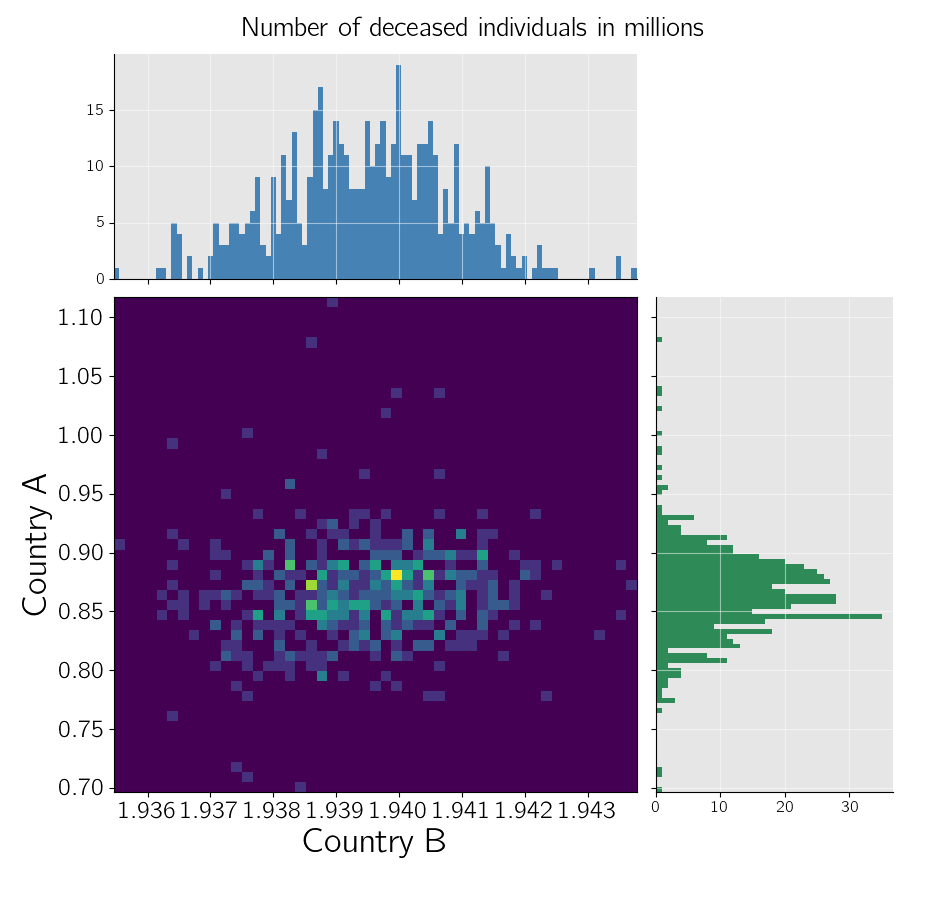
\includegraphics[width=\textwidth]{images/piecewise_stochastic_histogram_deceased_unrestricted.png}
         \caption{Unrestricted strategy}
         \label{fig:2d_unrestricted_piecewise}
     \end{subfigure}
     \hfill
     \begin{subfigure}[b]{0.49\textwidth}
         \centering
         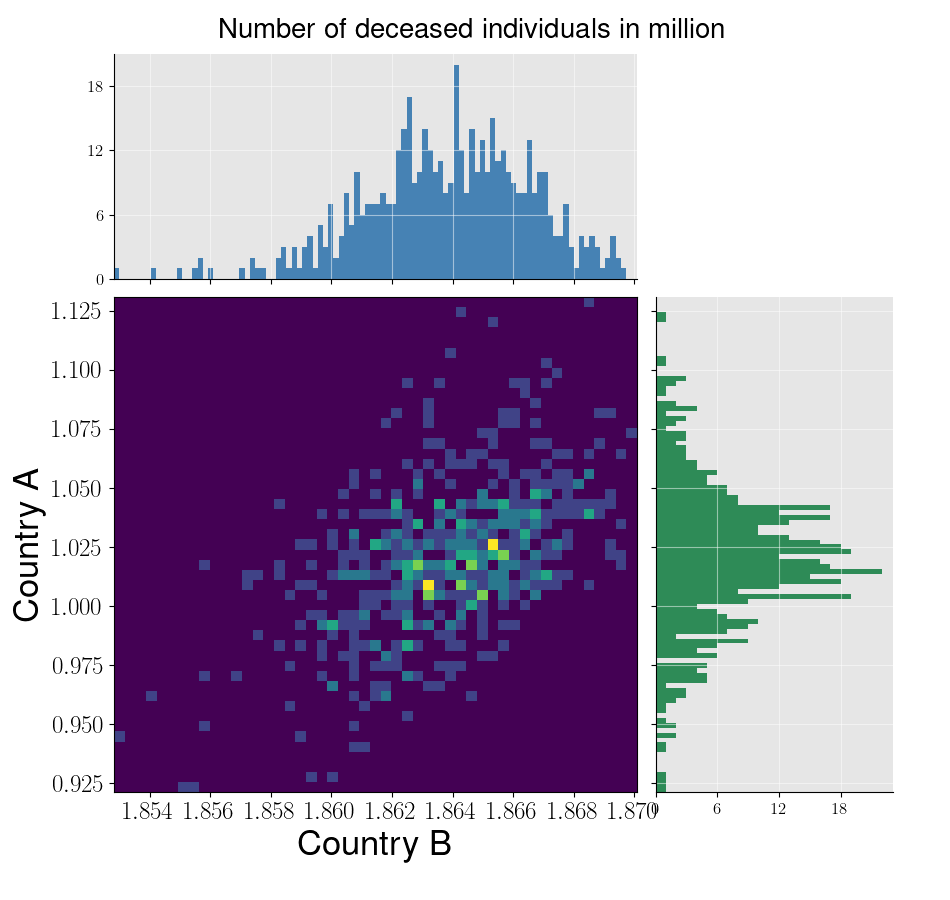
\includegraphics[width=\textwidth]{images/piecewise_stochastic_histogram_deceased_optimal.png}
         \caption{Pareto optimal strategy}
         \label{fig:2d_optimal_piecewise}
     \end{subfigure}
     \\
     \begin{subfigure}[b]{0.49\textwidth}
         \centering
         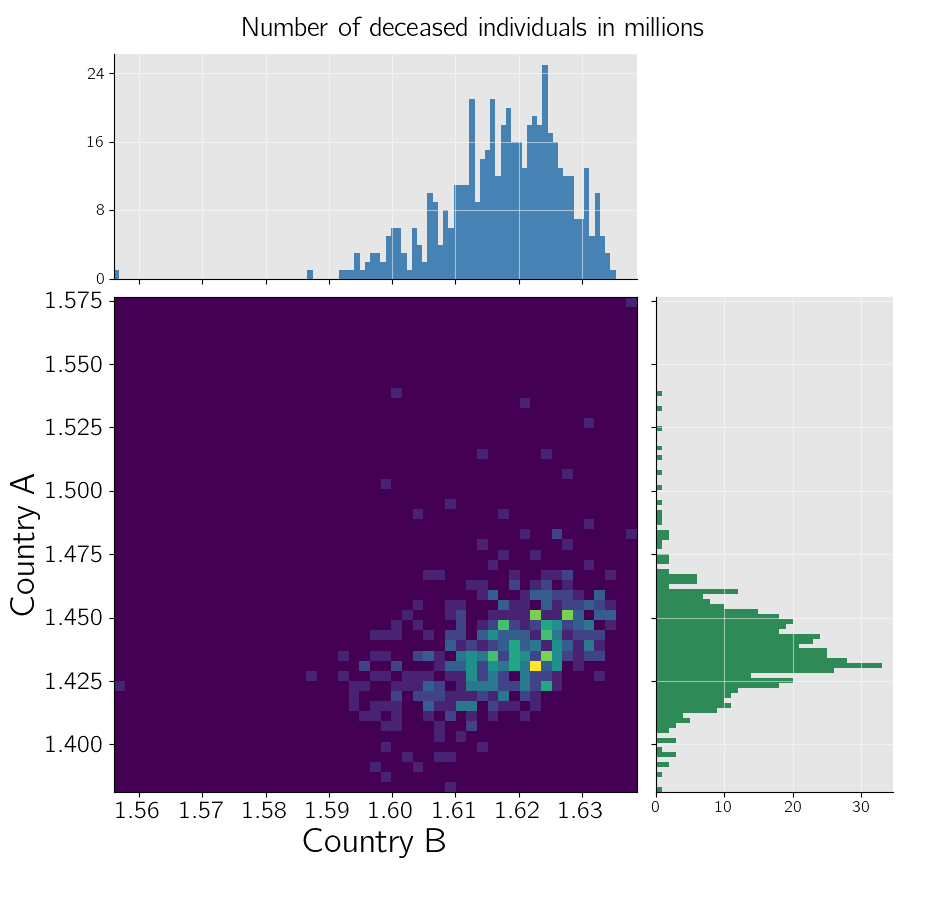
\includegraphics[width=\textwidth]{images/piecewise_stochastic_histogram_deceased_current.png}
         \caption{Current strategy}
         \label{fig:2d_piecewise}
     \end{subfigure}
\begin{flushleft}
\scriptsize{Note:} Purple temperature boxes indicate the joint frequencies. Histograms on top are the histograms corresponding to country B and histograms at the right-hand side are the histograms corresponding to country A. Histograms are computed using 500 simulations of the stochastic model using the Policies derived from splines. 
\end{flushleft}
        \caption{Frequencies of number of deceased individuals using strategies (Stepwise)}
        \label{fig:histograms_piecewise} 
\end{figure}

\clearpage
\subsection{Calculations and proofs}
We provide calculations and proofs that enhance our line of argumentation but would disturb the train of reading within the main section.
\subsubsection{Meeting probabilities}
\label{A:meeting_prob}
Using Bayes formula, we can rewrite the conditional probability as follows
\begin{align}
\label{eq:cond_meeting_prob}
&\quad \   \prob_t(i_2 \in \set(X_S, C_j, F_2)|i_1 \in \set(\neg X_D, C_A)) \\ &= \prob_t(i_2 \in \set(\neg X_D, C_j, F_2) | i_1 \in \set(\neg X_D, C_A) )  \notag \\
& \quad \cdot \prob_t(i_2 \in \set(X_S) | i_1 \in \set(\neg X_D, C_A), i_2 \in \set(\neg X_D, C_j, F_2) ) \notag \\
&= \prob_t(i_2 \in \set(\neg X_D, C_j, F_2) | i_1 \in \set(\neg X_D, C_A) )  \notag \\
& \quad \cdot \prob_t(i_2 \in \set(X_S)|i_2 \in \set(\neg X_D, C_j, F_2)  \notag
\end{align} 
We use the relative number of susceptible individuals $\set(X_S, C_j, F_2)$ across all individuals of $\set(\neg X_D, C_j, F_2)$ as approximation of the probability at the second line of the right-hand side 
\begin{align}
 \prob_t(i_2 \in \set(X_S, F_2)|i_2 \in \set(\neg X_D, C_j, F_2) ) = \frac{\num(X_S, C_j, F_2)}{\num(\neg X_D, C_j, F_2)}.
\end{align}

To account for the origin of $i_1$ within the first line of the right hand-side, we distinguish between the cases where $i_2 \in \set(C_A)$ and $i_2 \in \set(C_B)$. Assume that $i_2 \in \set(X_S, C_B, F_2)$. If there were no spatial effects to influence the cross-border meeting frequency we would use the unconditional probability 
\begin{align}
\prob_t(i_2 \in \set(\neg X_D, C_j, F_2)) = \frac{\num(\neg X_D, C_j, F_2)}{ \num(\neg X_D)}.   
\end{align}
To account for the spatial effects, we introduce a penalty function $b: \R_+ \to [0,1]$ that depends on the distances between both countries $d(A, B)$
\begin{align}
\label{eq:prob_cross_border}
\prob_t(i_2 \in \set(\neg X_D, C_B, F_2) | i_1 \in \set(\neg X_D, C_A) ) = \prob_t\left(i_2 \in \set(\neg X_D, C_B, F_2)\right) \cdot b(d(A, B)),
\end{align}

Yielding
\begin{align}
\label{eq:cond_meeting_prob_b}
\prob_t(i_2 \in \set(X_S, C_B, F_2)|i_1 \in \set(\neg X_D, C_A)) &= \frac{\num(X_S, C_j, F_2)}{\num(\neg X_D)} \cdot b(d(A, B))
\end{align} 


\subsubsection{Well-conditioning of the polynomial basis}
\label{A:well_conditioning}
First note that $B_1(0) = 1$ and $B_2(0), B_3(0), B_4(0) = 0$. Furthermore, $B_1(1), B_2(1), B_4(1) = 0$ and $B_3(1) = 1$. We first compute the function values at the boundaries $t_{i-1}$ and $t_i$.
\begin{align*}
P_{l,i}(t_{i-1}) &= B_1(0) P_{l,i}(t_{i-1}) + B_2(0) (t_{i} - t_{i-1}) P'_{l,i}(t_{i-1})  \\& \quad + B_3(0) P_{l,i}(t_{i}) + B_4(0) (t_{i} - t_{i-1}) P'_{l,i}(t_{i}) \\
&=  1 \cdot P_{l,i}(t_{i-1}) + 0 \cdot (t_{i} - t_{i-1}) P'_{l,i}(t_{i-1})  \\& \quad + 0 \cdot P_{l,i}(t_{i}) + 0 \cdot (t_{i} - t_{i-1}) P'_{l,i}(t_{i})\\
&= P_{l,i}(t_{i-1}) 
\end{align*}
\begin{align*}
P_{l,i}(t_{i}) &= B_1(1) P_{l,i}(t_{i-1}) + B_2(1) (t_{i} - t_{i-1}) P'_{l,i}(t_{i-1})  \\& \quad + B_3(1) P_{l,i}(t_{i}) + B_4(1) (t_{i} - t_{i-1}) P'_{l,i}(t_{i}) \\ 
&= 0 \cdot P_{l,i}(t_{i-1}) + 0 \cdot (t_{i} - t_{i-1}) P'_{l,i}(t_{i-1})  \\& \quad + 1 \cdot  P_{l,i}(t_{i}) + 0 \cdot (t_{i} - t_{i-1}) P'_{l,i}(t_{i})  \\
&= P_{l,i}(t_{i})
\end{align*}

The derivatives of the basis polynomials are 
\begin{align*}
B_1'(t) &= 6t^2 - 6t \\
B_2'(t) &= 3t^2 - 4t + 1 \\
B_3'(t) &= -6t^2 + 6t \\
B_4'(t) &= 3t^2 - 2t
\end{align*}
with $B_1(0)'=B_3(0)'=B_4(0)'=0$ and $B_2(t)'=\frac{1}{t_i - t_{i-1}}$. Moreover, $B_1'(1)'= B_2(1)'=B_3(1)'=0$ and $B_4(1)'=\frac{1}{t_i - t_{i-1}}$. The derivative of the polynomial is simply
\begin{align*}
P_{l,i}'(t) &= B_1'(t') P_{l,i}(t_{i-1}) + B_2'(t') (t_{i} - t_{i-1}) P'_{l,i}(t_{i-1})  \\& \quad + B_3'(t') P_{l,i}(t_{i}) + B_4'(t') (t_{i} - t_{i-1}) P'_{l,i}(t_{i})
\end{align*}
and therefore
\begin{align*}
P_{l,i}'(t_{i-1}) &= B_1'(0) P_{l,i}(t_{i-1}) + B_2'(0) (t_{i} - t_{i-1}) P'_{l,i}(t_{i-1})  \\& \quad + B_3'(0) P_{l,i}(t_{i}) + B_4'(0) (t_{i} - t_{i-1}) P'_{l,i}(t_{i}) \\
&= 0 \cdot P_{l,i}(t_{i-1}) + \frac{1}{t_i - t_{i-1}} \cdot(t_{i} - t_{i-1}) P'_{l,i}(t_{i-1})  \\& \quad + 0 \cdot P_{l,i}(t_{i}) + 0 \cdot (t_{i} - t_{i-1}) P'_{l,i}(t_{i}) \\
&=  P'_{l,i}(t_{i-1})
\end{align*}
and 
\begin{align*}
P_{l,i}'(t_{i-1}) &= B_1'(1) P_{l,i}(t_{i-1}) + B_2'(1) (t_{i} - t_{i-1}) P'_{l,i}(t_{i-1})  \\& \quad + B_3'(1) P_{l,i}(t_{i}) + B_4'(1) (t_{i} - t_{i-1}) P'_{l,i}(t_{i}) \\
&= 0 \cdot P_{l,i}(t_{i-1}) + 0 \cdot(t_{i} - t_{i-1}) P'_{l,i}(t_{i-1})  \\& \quad + 0 \cdot P_{l,i}(t_{i}) + \frac{1}{t_i - t_{i-1}} \cdot (t_{i} - t_{i-1}) P'_{l,i}(t_{i}) \\
&=  P'_{l,i}(t_{i}).
\end{align*}

\subsubsection{Convergence in distribution}
\label{A:convergence_distribution}
%\begin{theorem}
%$\textrm{B}\left(\frac{\tau}{dt}, a_j(y) \cdot dt\right) \xrightarrow{d} \textrm{Po}(a_j(y) \cdot \tau)$ if $dt \to 0$.
%\end{theorem}
\Poisson*
\begin{proof}
Let $p_n$ be a sequence with $\lim_{n \to \infty} p_n = 0$. We first show that if $\lambda'=n \cdot p_n$ is constant, $n \to \infty$ and $p_n \to 0$, a general Binomial random variable $\textrm{B}(n, p_n)$ converges in distribution to a Poisson random variable $\textrm{Po}(\lambda')$. Note that this proof is in essence just a restatement of the Poisson limit theorem of \cite{Poisson.1835}.
\begin{align*}
\lim_{n \to \infty} \binom{n}{k} p^k_n (1-p_n)^{n-k} &= \lim_{n \to \infty} \frac{n \cdot (n-1) \cdot \hdots \cdot (n-k+1)}{k!} \left(\frac{\lambda'}{n} \right)^k \left(1-\frac{\lambda'}{n} \right)^{n-k} \\
&= \lim_{n \to \infty} \frac{n^k + O(n^{k-1})}{k!} \left(\frac{\lambda'}{n} \right)^k \left(1-\frac{\lambda'}{n} \right)^{n-k} \\
&= \frac{\left(\lambda'\right)^k}{k!} \exp{(-\lambda')}
\end{align*}
Note that by definition $\tau$ is fixed and by assumption $a_i(y)$ is constant within $[t, t+\tau)$. Thus, $\lim_{dt \to 0} \frac{\tau}{dt} = \infty$, $\lim_{dt \to 0} a_i(y) \cdot dt = 0$ and $\frac{\tau}{dt} \cdot a_i(y) \cdot dt = \tau \cdot a_i(y)$. Using the convergence property mentioned above yields the result.
\end{proof}


\subsubsection{Polynomial basis}
\label{A:polynomial_basis}
\Basis*
\begin{proof}
We need to show that the four polynomials are linearly independent. We do so by writing the polynomials in vector form, collect them in a matrix and show that this matrix has full rank. 
\begin{align*}
\begin{pmatrix}
2 & 1 & -2 & 1\\
-3 & -2 & 3 & -1 \\
0 & 1 & 0 & 0 \\
1 & 0 & 0 & 0 \\
\end{pmatrix}
\Leftrightarrow
\begin{pmatrix}
0 & 0 & -2 & 1\\
0 & 0 & 1 & -1 \\
0 & 1 & 0 & 0 \\
1 & 0 & 0 & 0 \\
\end{pmatrix}
\Leftrightarrow
\begin{pmatrix}
0 & 0 & 0 & -1\\
0 & 0 & 1 & -1 \\
0 & 1 & 0 & 0 \\
1 & 0 & 0 & 0 \\
\end{pmatrix}
\Leftrightarrow
\begin{pmatrix}
0 & 0 & 0 & 1\\
0 & 0 & 1 & 0 \\
0 & 1 & 0 & 0 \\
1 & 0 & 0 & 0 \\
\end{pmatrix}
\end{align*}
Since $B_1(t), B_2(t), B_3(t), B_4(t)$ are four linearly independent polynomials of degree 3, they form a basis of $\R_3(t)$. 
\end{proof} 
